In boundary defense with heterogeneous defenders (\prob), there are $k$ defenders (which may be robots and/or other types of agents) with speeds $v_1,\dots,v_k$, where each defender is modeled as a point in some domain $\mathcal E = \mathbb R^2$ or $\mathbb R^3$.
The defenders live on a lower dimensional subspace of $\mathcal E$ (i.e., some boundary of a subset of $\mathcal E$).  
There are also $n$ attack events $\big\langle loc_i, t_i\big\rangle_{i=1}^{n}$, where each attack event is a pair $\big\langle loc, t\big\rangle$ in which $loc$ is the
location of the attack and $t$ is the time it happens. 
The $i^{{th}}$ attack is intercepted by a defender only if the defender is located at $loc_i$ at time $t_i$.
For initialization, we denote the initial locations of the $k$ defenders at $t=0$ as $loc^{1},\dots, loc^{k}$. 

Following the definition in \cite{adler2022role}, we define the horizon of the defenders as follows,
\begin{definition}[Horizon]
The (look ahead) \textit{horizon} $T$ of the defenders is defined as the amount of time defenders can peek into the attack sequence in the future. That is, given the current time $t$, and a horizon $T$, defenders have access to complete information on attacks happening on or before $t+T$. 
\end{definition}

Now, we provide formulations of the two versions of the \prob problem studied in this paper. In the infinite horizon setting, $T = \infty$, all attack events are given in a single batch.

\begin{problem}[Infinite-horizon \prob]\label{prob:bd-1}
Given $k$ defenders with speed $v_1, \dots, v_k$ and initial locations $loc^1, \ldots, loc^k$, and $n$ attack events $\big\langle loc_i, t_i\big\rangle_{i=1}^{n}$, intercept as many attacks as possible. 
\end{problem}

In a finite-horizon setting, the attack events are not all revealed at $t=0$ but are given as a stream of attacks $\big\langle loc_i, t_i\big\rangle_{i=1}^{\infty}$. The defenders can only know the attack events within a horizon or time window of $T < \infty$ in the future.

\begin{problem}[Finite-horizon \prob]\label{prob:bd-2}
There are $k$ defenders with speed $v_1, \dots, v_k$ and initial locations $loc^1, \ldots, loc^k$, and a stream of attack events.
%
At each time instance $t$, the defenders only know attack events happening no later than time $T$ in the future (i.e. $t_i \le t+T$).
%
Intercept as many attacks as possible. 
\end{problem}

We introduce here two useful notations: $next(a, d)\ (a\in[0, n],\ d\in[1,k])$ and $prev(a, d)\ (a\in[1,n],\ d \in [1,k])$.
They are defined as
\begin{align}
next(a, d) = \{ a'| dist(loc_a, loc_{a'}) \leq v_d \cdot (t_{a'} - t_a) \}    \\
prev(a, d) = \{ a'| dist(loc_a, loc_{a'}) \leq v_d \cdot (t_a - t_{a'}) \}    
\end{align}
where $dist(x,y)$ denotes the distance between location $x$ and $y$. 
In other words, $next(a, d)$ is the set of 
attack events that can be reached from the location of the $a^{th}$ attack event by defender $d$. 
And $prev(a,d)$ is the set of attack events from whose location defender $d$ can reach the $a^{th}$ attack event. 
Additionally, $next(0, d)$ denotes the set of attack events that can be reached by defender $d$ from its initial location.
Similarly, $prev(a, d)$ contains $0$ if defender $d$ can reach the location of attack $a$ from its initial location.
~\ref{fig:bd-next_prev} gives an example for defender $1$.

\begin{figure}[h]
    \centering
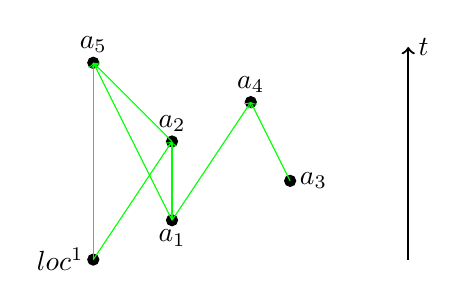
\begin{tikzpicture}
%\draw[black, thick, ->] (0,0) -- (4.5,0) node[anchor=south]{location};
\draw[black, thick, ->] (5,0) -- (5, 2.7) node[anchor=west]{$t$};

\filldraw[black] (1, 0) circle (2pt) node[anchor=east](iloc1){$loc^1$};

\filldraw[black] (2,0.5) circle (2pt) node[anchor=north](a1){$a_1$};
\filldraw[black] (2,1.5) circle (2pt) node[anchor=south](a2){$a_2$};
\filldraw[black] (3.5,1) circle (2pt) node[anchor=west](a3){$a_3$};
\filldraw[black] (3,2) circle (2pt) node[anchor=south](a4){$a_4$};
\filldraw[black] (1,2.5) circle (2pt) node[anchor=south](a5){$a_5$};

\draw[green, thin, ->] (iloc1.east) -- (a2.south);
\draw[green, thin, ->] (iloc1.east) -- (a5.south);

\draw[green, thin, ->] (a1.north) -- (a2.south);
\draw[green, thin, ->] (a1.north) -- (a4.south);
\draw[green, thin, ->] (a1.north) -- (a5.south);
\draw[green, thin, ->] (a2.south) -- (a5.south);
\draw[green, thin, ->] (a3.west) -- (a4.south);

\end{tikzpicture}
    \caption{Illustration of an example of reachability between different attack events for defender $1$.  
    For example, $next(1, 1) = \{2,4,5\}$, $next(0,1)=\{2,5\}$, $prev(2, 1) =\{0, 1\}$, $prev(1,1)=\varnothing$.
    $loc^1$ cannot reach $a_1$ since $v_1$ is not sufficiently large. For the same reason, defender $1$ cannot reach $a_3$ from $a_1$.
    }
    \label{fig:bd-next_prev}
\end{figure}

